\chapter{Soft CGRA Overlay Based FPGA Accelerator} \label{chapter:overlay}
Instead of developing random applications on FPGA, this work targets a hybrid CPU-FPGA computing system while it offloads the compute intensive loop kernels to the FPGA for performance acceleration and leaves the rest of the control intensive part on the CPU. \figref{fig:hls-accelerator} shows the design of a typical FPGA accelerator system. In such a system, on-chip memory is used to buffer data between the host CPU and the accelerator. A controller is also presented in hardware to control the operations of the accelerator as well as memory transfers. The controller attached to the system interconnection works at a separate clock domain with lower frequency. The entire design must be reimplemented every time a change is made to the accelerator design, going through the lengthy low-level hardware implementation tool flow. 

On the other hand, \figref{fig:scgra-accelerator} shows the system generated on top of SCGRA overlay. While it features a similar overall design as a typical accelerator system, it utilizes a regular SCGRA overlay instead of irregular random logic to implement the computation and the overlay can be reused during the design iterations or within a domain of applications. The SCGRA consists of an array of simple processing elements (PEs) connected by a direct network executing synchronously. Each PE computes and forwards data in lock steps, allowing deterministic multi-hop data communication that overlaps with computations. The action of each PE in each cycle is controlled by an instruction ROM that is populated with instructions generated by the compiler. Finally, a data memory is featured on each PE to serve as a temporary storage for run-time data that may be reused in the same PE or be forwarded in subsequent steps. Communication between the accelerator and the host processor is carried through a group of input/output buffers. Accesses to these I/O buffers from the SCGRA array take place in lock step with the rest of the system. The exact buffer location to be accessed is control by the AddrIBuf and AddrOBuf blocks. Both of them are ROM populated with address information generated from the SCGRA compiler which will be detailed in the next chapter. Finally, the kernel CGRA computing logic may repeat the same computing a number of times on a block of data stored in input buffer i.e. IBuf. For that, an additional CGRACtrl block is used to translate the controlling signals from AccCtrl block.   

\begin{figure}
\centering
\subfigure[Conventional FPGA Accelerator]{
\includegraphics[width=0.47\linewidth]{hls-accelerator}
\label{fig:hls-accelerator}
}
\hfill
\subfigure[SCGRA Based FPGA Accelerator]{
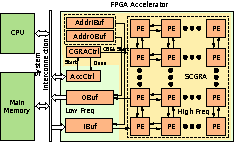
\includegraphics[width=0.47\linewidth]{scgra-accelerator}
\label{fig:scgra-accelerator}
}
\caption{Hybrid CPU-FPGA Computation System}
\label{fig:FPGA-accelerator}
\end{figure}

One key factor that determines the accelerator's performance rests on the design of the SCGRA overlay. In particular, the accelerator will not be as useful without significant performance speedup. For that, the overlay should be \emph{reconfigurable} so that it can be rapidly customized specifically to an application or a domain of application for higher performance as well as energy efficiency. Meanwhile, the SCGRA overlay must be highly \emph{pipelined} and make best use of the underlying FPGA fabrics to work at high frequency. In addition, the SCGRA overlay should also be \emph{deterministic} for the sake of efficient lock-step computing. 

\section{Reconfiguration}
There are two levels of reconfiguration that may be applied to the overlay to address different application needs. The first and the quickest form of reconfiguration keeps the physical implementation of the overlay intact. To modify the function of the implemented hardware, the SCGRA overlay can be configured by changing (i) the content of the instruction ROM of each PE, (ii) the content of the input/output buffer, (iii) the content of the I/O buffer address ROM AddrIBuf and AddrOBuf, and (iv) the accelerator control AccCtrl.  Among these 4 aspects, (i) and (iii) are modified by replacing the ROM content of the bitstream in-place using tools such as \texttt{data2mem}. On the other hand (ii) and (iv) are controlled by software during run-time.  As a result, all 4 types of customization can be performed rapidly within seconds. They allow the same overlay implementation to be targeted to different applications as well as to different loop iterations of the compute kernel easily.

A second level of customization can be applied to the overlay implementation itself. As a \emph{soft} overlay, many aspects of the array can be customized according to the input application to achieve different tradeoffs in area, energy and performance. Customizations may involve, the size of the array, the type of supported operation in each PE, the size of data and instruction memory, and even the pipeline depth of the network and the PEs. When compared to the first level of customization, this level of customization involves reimplementation of the overlay and requires considerably longer run time. User may therefore opt for this level of customization only as needed. Note that in all cases, the overlay remains synchronous and deterministic to keep the overall flow of QuickDough intact.

\section{Processing Element (PE)}
The key design element of the CGRA overlay is its processing element (PE). On one hand, the design of the PE must be simple with low overhead to reduce area and energy consumption, and to improve performance. On the other hand, the design of PE must also be flexible enough that it can support all the required operations in the target application.

\begin{figure}
\center{\includegraphics[width=0.6\linewidth]{pe}}
\caption{Fully pipelined PE structure. Each PE can be connected to at most 4 neighbours.}
\label{fig:pe}
\end{figure}

\figref{fig:pe} shows the current implementation of a PE that features an optional load/store path. At the heart of the PE is an ALU, which is supported by a multi-port data memory and an instruction memory. Three of the data memory's read ports are connected to the ALU as inputs, while the remaining ports are sent to the output multiplexors for connection to neighboring PEs and the optional store path to OBuf external to the PE. At the same time, this data memory takes input from the ALU output, data arriving from neighboring PEs, as well as from the optional IBuf loading path. The action of the PE is controlled by the AddrCtrl unit that reads from the instruction memory. Finally, a global signal from the AccCtrl block controls the start/stop of all PEs in the array.

\subsection{Instruction Memory and Data Memory}
The instruction memory stores all the control words of the PE. As its content does not change at run-time, a ROM is used to implement this instruction memory. As shown in \figref{fig:inst-rom}, the address of the instruction memory is generated using a counter controlled by the \texttt{CGRAStart} from CGRACtrl block. Once the \texttt{CGRAStart} signal is valid, the instruction memory address will increase by one every cycle and the SCGRA execution will proceed accordingly. When the \texttt{CGRAStart} signal is invalid, the address will be reset to be 0 and the SCGRA execution will stop. In addition, pipeline registers are added to the output port of the instruction memory to ensure high implementation frequency.

\begin{figure}
\center{\includegraphics[width=0.5\linewidth]{inst-rom}}
\caption{Instruction Memory}
\label{fig:inst-rom}
\end{figure}

Data memory stores intermediate data that can either be forwarded to the neighboring PEs or be sent to the ALU for calculation. To support non-blocking operations in the PE, at least 4 read and 2 write ports are needed. In each cycle, 3 reads are needed for the ALU and 1 read is needed for data forwarding. At a single cycle, one write port is needed to store input data from neighboring PEs and another one is needed to store the computing result of the ALU within the same cycle. The structure of the data memory is shown in \figref{fig:data-mem}. In order to achieve high implementation frequency and meet various data memory capacity requirements, instead of using highly multiplexed flip flops, 3 primitive true dual port memory blocks that contain replicated data are employed to implement this data memory. The three BRAMs share 2 R/W selection lines for all the ports. It has two write ports and six read ports literally, but one write port and corresponding set of three reading ports are not allowed to act at the same cycle. For instance, when write port0 is selected, read port0, read port2 and read port4 are inactive. Compared to a standard 2-write-6-read multi-ported memory which allows 8 parallel read/write operations \cite{abdelhadi2014modular}, it makes best use of the primitive block RAMs on FPGAs saving the resource consumption and achieving better timing. 

\begin{figure}
\center{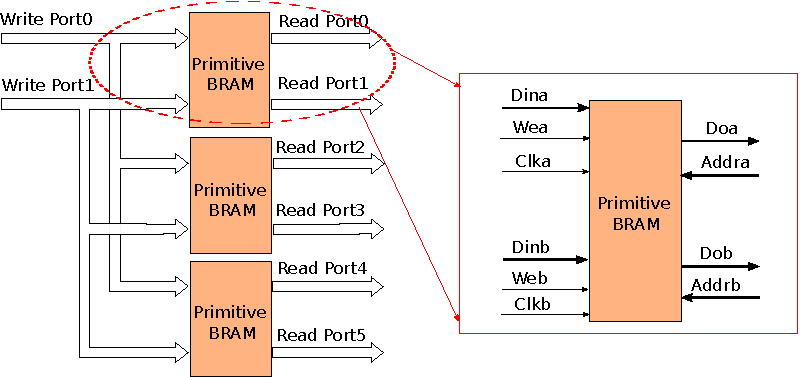
\includegraphics[width=0.7\linewidth]{data-mem}}
\caption{Multi-ported Data Memory, It makes best use of the primitive block RAM on FPGAs, though the read ports and write ports in the same group (e.g. Doa, Addra and Dina, Wea, Clka belong to the same group) are not allowed to act in parallel.}
\label{fig:data-mem}
\end{figure}

\subsection{ALU}
At the heart of the proposed PE is the ALU that carries out the computations of the given application.  As an overlay, the SCGRA overlay ALU must be simple, regular, and flexible such that it may easily be customized with different operations specifically for any given user application.  In addition, it must also be fully pipelined in order to achieve high clock frequency and thus higher overall performance. \figref{fig:ALU} shows the current design of the ALU used in the SCGRA overlay.

\begin{figure}
\center{\includegraphics[width=0.49\linewidth]{alu}}
\caption{ALU of the SCGRA Overlay. It supports up to 16 fully pipelined 3-input operations.}
\label{fig:ALU}
\end{figure} 

The ALU supports up to 16 fully pipelined 3-input operations.  Depending on the area-performance requirements, the ALU may be customized with operations specifically designed for the application.  It may also be customized to support the common set of operations for multiple compute kernels. For example, \tabref{tab:operations} shows the set of operations we have developed for all the benchmarks in the experiment. \figref{fig:ALU} shows the current set of operation. These operators in the ALU may execute concurrently in a pipelined fashion and must complete in a deterministic number of cycle.  Given the deterministic nature of the operators, the SCGRA scheduler will ensure that there is never conflict at the output multiplexor.

\begin{table}
\footnotesize
\centering
\caption{Operation Set Implemented in ALU. It covers all the four applications used in the experiments.
\label{tab:operations}}{
\footnotesize 
\centering
\begin{tabular}{l|c|l}
\hline
Type & Opcode & Expression \\

\hline
MULADD & 0001 & {Dst = (Src0 $\times$ Src1) + Src2} \\

\hline
MULSUB & 0010 & {Dst = (Src0 $\times$ Src1) - Src2} \\

\hline
ADDADD & 0011 & {Dst = (Src0 + Src1) + Src2} \\

\hline
ADDSUB & 0100 & {Dst = (Src0 + Src1) - Src2} \\

\hline
SUBSUB & 0101 & {Dst = (Src0 - Src1) - Src2} \\

\hline 
PHI & 0110 & {Dst = Src0 ? Src1 : Src2} \\

\hline
RSFAND & 0111 & {Dst = (Src0 $\gg$ Src1) \& Src2} \\

\hline
LSFADD & 1000 & {Dst = (Src0 $\ll$ Src1) + Src2} \\

\hline
ABS & 1001 & {Dst = abs(Src0)} \\

\hline
GT & 1010 & {Dst = (Src0 $>$ Src1) ? 1 : 0} \\

\hline
LET & 1011 & {Dst = (Src0 $\leq$ Src1) ? 1 : 0} \\

\hline
ANDAND & 1100 & {Dst = (Src0 \& Src1) \& Src2} \\

\hline
\end{tabular}
}
\end{table}

\subsection{Load/Store Interface}
For the PEs that also serve as IO interface to the SCGRA, they have an additional load path and a store path as shown in \ref{fig:pe}. The data loading path and the SCGRA neighboring input share a single data memory write port, and an additional pipeline stage is added to keep the balance of the pipeline. Similarly, the data storing path has an additional data multiplexers as well, but it doesn't influence the pipeline of the design. 

To improve the performance of the resulting SCGRA overlay based accelerators, the load/store address calculation of the compute kernels is done in the QuickDough compiler. The addresses are generated at compilation time and then stored in the AddrIBuf and AddrOBuf. Consequently, there is only pure data in the load/store path while 1 bit \texttt{LoadValid} signal and 1 bit \texttt{StoreValid} signal are used to obtain the addresses from the address buffers i.e. AddrIBuf and AddrOBuf.

\section{Accelerator Buffers}
Input/output buffer is used to store data transmitted between the FPGA accelerator and main memory. Since the two ports of the input/output buffers are either specialized as input or output (For instance, the input buffer has one write only port connected to the system interconnection while they have the other read only port connected to the SCGRA computing logic.), simple dual port block RAMs can be used to implement the input/output buffers. 

The input/output address buffers store the addresses of load/store operations. As these addresses are decided at compilation time, the input/output buffers are implemented as ROM. While the addresses of load/store operations are stored in the same sequence as the load/store sequence. In order to return the required addresses upon to the \texttt{LoadValid}/ \texttt{StoreValid} signal, the ROM relies on a counter to generate the ROM reading addresses, which is similar to the instruction memory of each PE. 

\section{Accelerator Controller}
AccCtrl starts the lock-step computing of the whole SCGRA array when it receives the \texttt{start} signal from the host processor. At the end of the computing, \texttt{done} signal will be sent to the host processor to collect the computing result. Since the regular SCGRA overlay typically runs at higher frequency than the interface connected to the system interconnection, they are allocated in two separate clock domains, and the \texttt{start} and \texttt{done} transmit across the two clock domains through three-level registers.

On top of the basic features, the accelerator allows the CGRA computing logic to be repeated on data transmitted through the input/output buffers, which helps to amortize the initial data transfer cost. To support this unique feature, CGRACtrl has two registers \texttt{ItNum} and \texttt{ItLen} to represent the number of the repeated CGRA computing and the length of each compute iteration. Based on the two registers, CGRACtrl produces the \texttt{CGRAStart} signal which controls the action of the instruction memory and the \texttt{Done} signal that indicates the end of the hardware execution. 

\section{Experiments}
SCGRA overlay is the backbone of the accelerator and its implementation is critical to the resulting FPGA acceleration system. Thus a series of experiments are conducted to evaluate the SCGRA overlay implementation in terms of pipelining and scalability which further exhibits the performance, power consumption and energy efficiency of the SCGRA overlay. This section is organized as follows. Basic experiment setup is presented in next subsection. Then the overlay pipelining and scalability are analyzed respectively. 

\subsection{Experiment Setup}
Both $2 \times 2$ and $5 \times 5$ SCGRA overlays were developed in ISE 14.7 and Vivado 2013.4 targeting XC7Z020 FPGA which is the FPGA on Zedboard. The overlays support all the operations as mentioned in previous section. 

In order to explore the SCGRA overlay pipelining, SCGRA overlays with different pipelining have been developed. As shown in \tabref{tab:pipeline-config}, the SCGRA overlay implementations with different pipelining configurations can typically run at 100MHz, 150MHz, 200MHz and 250MHz respectively. Note that \texttt{Input $\rightarrow$ Output} in \tabref{tab:pipeline-config} represents the latency of a normal data transmitting from input port of a PE to an output port of the PE. \texttt{Input $\rightarrow$ Bypass $\rightarrow$ Output} stands for the bypass data path length of a PE. \texttt{Input $\rightarrow$ Write Back} means data transmitting latency from input port of a PE to the write port of data memory in the PE. As it includes the latency of data paths of different operations in ALU, it varies while it remains deterministic for each specific operation. The rest part of the basic configurations of the overlay are shown in \tabref{tab:basic-config}. 

\begin{table}
\footnotesize
\caption{Pipeline Configurations \label{tab:pipeline-config}}{
\centering
\begin{tabular}{c|c|c|c}
\hline
{Pipeline Options} & {\texttt{Input $\rightarrow$ Output}} & \tabincell{l}{\texttt{Input $\rightarrow$ Bypass} \\ \texttt{$\rightarrow$ Output}} & {\texttt{Input $\rightarrow$ Write Back}} \\ \hline
{100MHz} & {2 cycles} & {1 cycle} & {4\~{}6 cycles} \\ \hline
{150MHz} & {2 cycles} & {1 cycle} & {5\~{}8 cycles} \\ \hline
{200MHz} & {4 cycles} & {2 cycles} & {7\~{}11 cycles} \\ \hline
{250MHz} & {7 cycles} & {3 cycles} & {11\~{}17 cycles} \\ \hline
\end{tabular}
}
\end{table}

\begin{table}
\footnotesize
\caption{SCGRA Configuration \label{tab:basic-config}}{
\centering
\begin{tabular}{c|c|c|c|c}
\hline
{SCGRA Topology} & {Instruction Memory} & {Data Memory} & {I/O Data Buffer} & {I/O Address Buffer} \\ \hline
{Torus} & {1K $\times$ 72 bits} & {$256 \times 32$ bits} & {2K $\times$ 32 bits} & {4K $\times$ 18 bits} \\ \hline
\end{tabular}
}
\end{table}

In order to estimate the performance of the overlays with different pipelining, a group of DFGs generated from matrix multiplication (MM), finite impulse filter (FIR), Sobel edge detector (SE), K-means (KM) with different configurations are mapped to the overlay as the benchmark. The configurations of the compute kernels are detailed in \tabref{tab:benchmark-config} and the extracted DFGs are presented in \tabref{tab:dfg-info}. 

\begin{table}
\footnotesize
\centering
  \caption{Detailed Configurations of the Benchmark 
  \label{tab:benchmark-config}}{
  \centering
  \begin{tabular}{l|l|l|l|l}
  \hline
  Benchmark & MM & FIR & SE & KM \\ \hline
  Configurations & Matrix Size & \tabincell{l}{\# of Input/\\ \# of Taps+1} & \tabincell{l}{ \# of Vertical Pixels/\\ \# of Horizontal Pixels} & \tabincell{l}{\# of Nodes/Centroids/\\Dimension} \\ \hline
  C1 & 10 & 40/50 & 8/8 & 20/4/2 \\ \hline
  C2 & 100 & 10000/50 & 128/128 & 5000/4/2 \\ \hline
  C3 & 1000 & 100000/50 & 1024/1024 & 50000/4/2 \\ \hline
  \end{tabular}
  }
\end{table}

\begin{table}
\footnotesize
\centering
  \caption{DFG Information (\# of Input/ \# of Output/ \# of Operations) 
  \label{tab:dfg-info}}{
  \centering
  \begin{tabular}{l|l|l|l|l}
  \hline
  Configurations & MM & FIR & SE & KM \\ \hline
  C1 & 200/100/1000 & 70/20/860 & 31/8/1080 & 49/12/920 \\ \hline
  C2 & 600/5/750 & 120/20/1000 & 31/8/1080 & 59/12/1144 \\ \hline
  C3 & 400/1/301 & 120/20/1000 & 27/4/540 & 59/12/1144 \\ \hline
  \end{tabular}
  }
\end{table}

\subsection{Pipelining}
Pipelining influences both the latency of the SCGRA overlay data paths and the implementation frequency of the resulting accelerators, which further affects the performance, resource consumption and the energy efficiency of the FPGA acceleration system. To explore the SCGRA overlay pipelining, this subsection focuses on how different SCGRA overlay pipelining affects the performance, resource consumption and energy efficiency of the resulting hardware accelerators. 

By using the benchmark \tabref{tab:benchmark-config} and \tabref{tab:dfg-info}, \figref{fig:pipeline-cycle-cnt} shows the relation between the SCGRA overlay pipelining and the number of DFG execution on both a $2 \times 2$ SCGRA overlay and a $5 \times 5$ SCGRA overlay. It is clear that SCGRA overlays with less pipeline stages and lower implementation frequency typically achieves shorter execution cycles due to the shorter data path as detailed in \tabref{tab:pipeline-config}. However, when taking the clock frequency in to consideration, SCGRA overlays with deeper pipelining and higher implementation frequency outperform eventually on the overall run-time as presented in \figref{fig:pipeline-run-time}. There are exceptions for example FIR C1 mapped to the $5 \times 5$ SCGRA overlay exhibits slightly differently. It is mainly caused by the operation scheduling which is essentially an NP-complete problem. When mapping a relatively small DFGs to a larger SCGRA, it will be challenging for the scheduler to compromise between the load balance and the communication cost and scheduling performance may fluctuate. The detailed operation scheduling will be further discussed in next chapter. In this case, using a smaller SCGRA overlay instead of a larger one usually solves this problem. In summary, fully pipelined SCGRA overlay will be used in QuickDough aiming to provide high-performance FPGA accelerators.

\begin{figure}[tb]
\centering
\subfigure[SCGRA$2 \times 2$]{
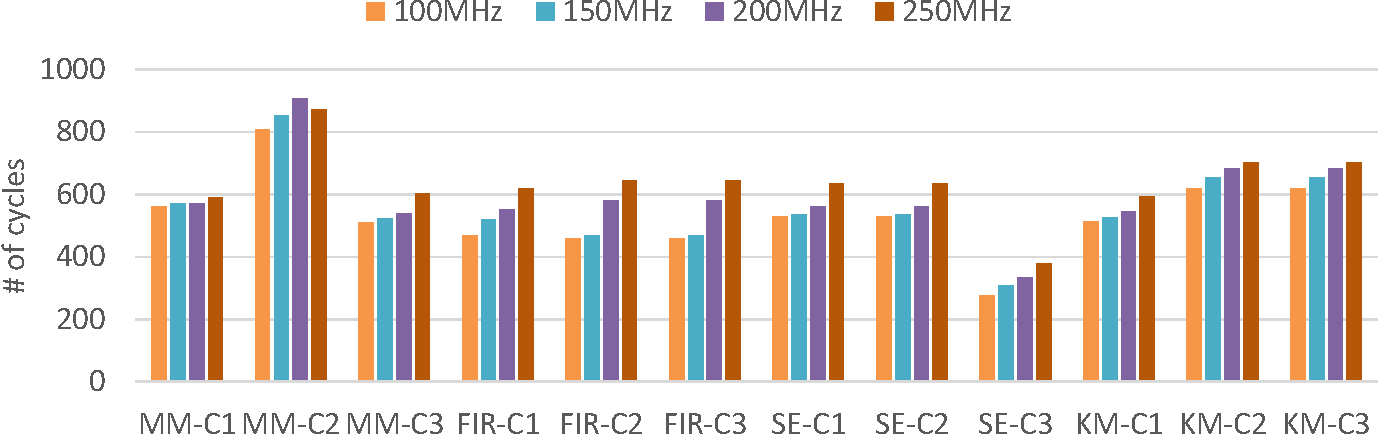
\includegraphics[width=0.8\linewidth]{pipeline-cgra2x2-sim-perf}
\label{fig:pipeline-cgra2x2-cycle-cnt}
}
\hfill
\subfigure[SCGRA $5 \times 5$]{
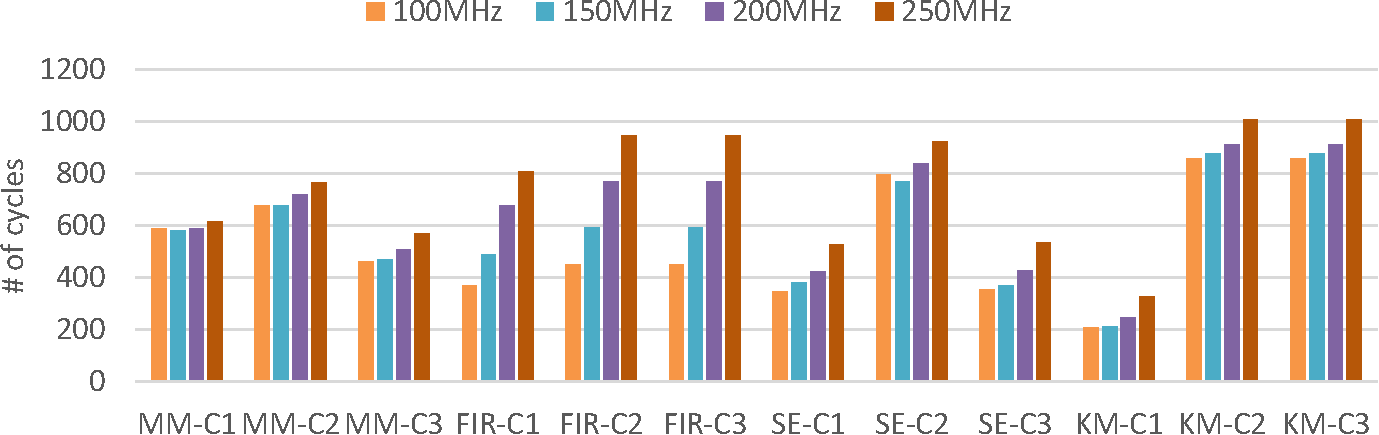
\includegraphics[width=0.8\linewidth]{pipeline-cgra5x5-sim-perf}
\label{fig:pipeline-cgra5x5-cycle-cnt}
}
\caption{The Number of Cycles of DFG Execution on SCGRA Overlays with Different Pipelining}
\label{fig:pipeline-cycle-cnt}
\end{figure}

\begin{figure}[tb]
\centering
\subfigure[SCGRA$2 \times 2$]{
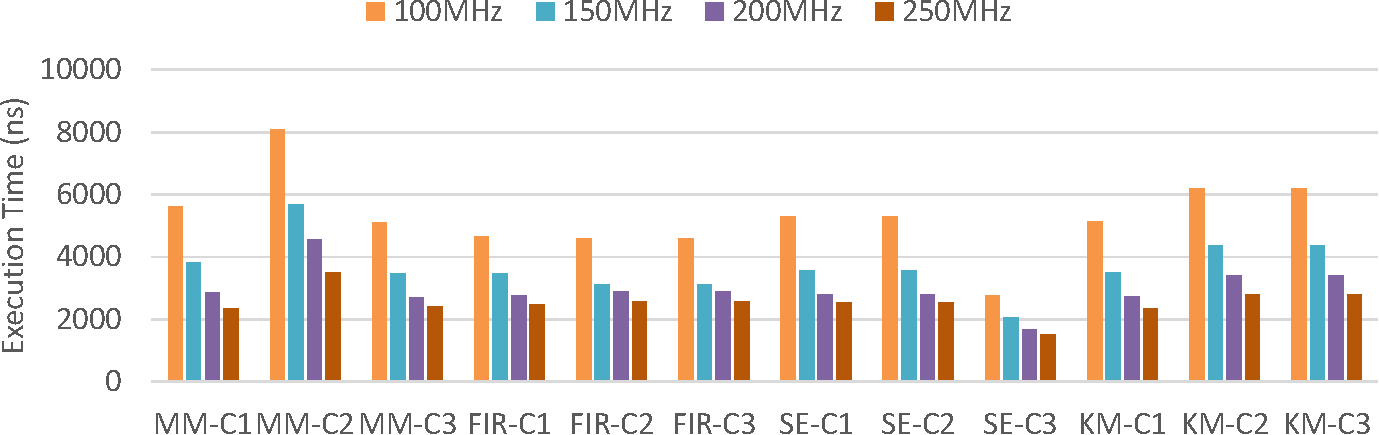
\includegraphics[width=0.8\linewidth]{pipeline-cgra2x2-real-perf}
\label{fig:pipeline-cgra2x2-run-time}
}
\hfill
\subfigure[SCGRA $5 \times 5$]{
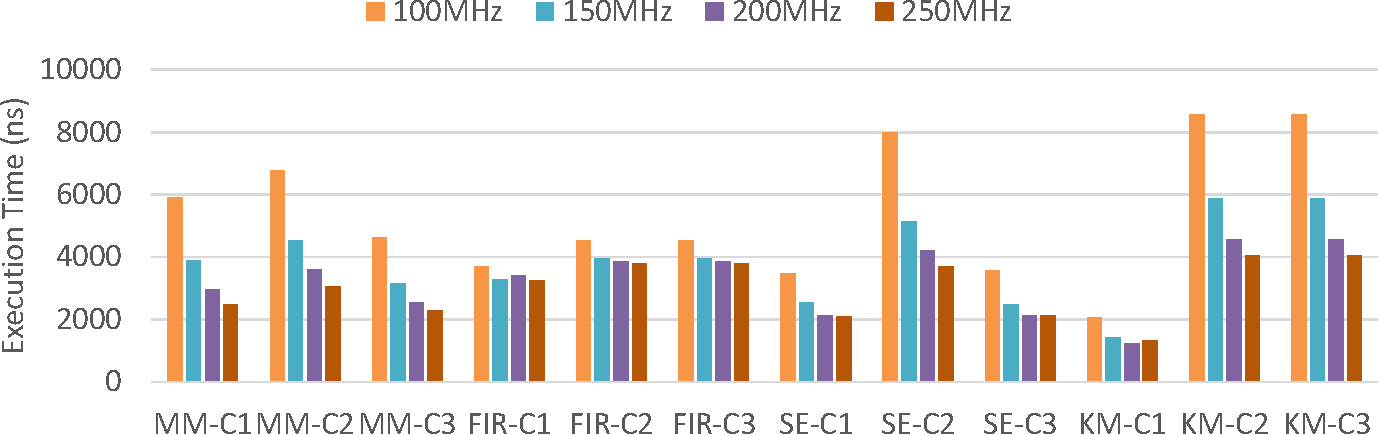
\includegraphics[width=0.8\linewidth]{pipeline-cgra5x5-real-perf}
\label{fig:pipeline-cgra5x5-run-time}
}
\caption{Overall DFG Execution Time on SCGRA Overlays with Different Pipelining}
\label{fig:pipeline-run-time}
\end{figure}

The SCGRA overlay pipelining also had direct influence on the FPGA resource consumption. \figref{fig:pipeline-resource} shows the hardware resource utilization of SCGRA overlay with different pipelining. It can be found that the overlays with deeper pipelining and higher implementation frequency consumes more Flip Flops (FFs) and slightly more LUTs while the RAM blocks and DSP slices remain the same. While the SCGRA overlays have rather low FFs and LUTs utilization, therefore deeper pipelining and higher implementation frequency typically will not bring significant resource constrain to the FPGA accelerator design. 

\begin{figure}[htb]
\center{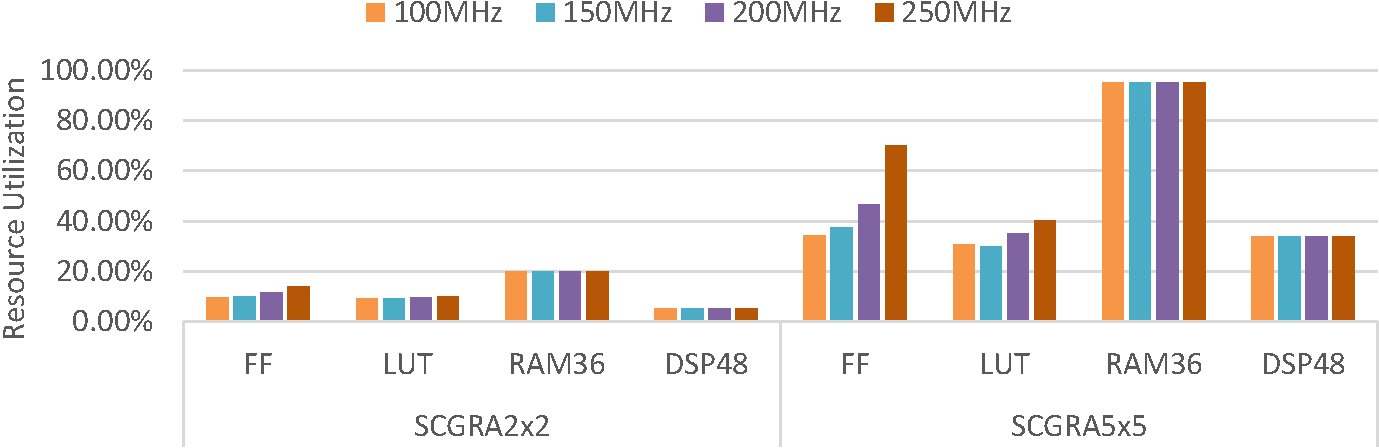
\includegraphics[width=0.8\linewidth]{pipeline-resource}}
\caption{Hardware Resource Utilization of SCGRA Overlays with Different Pipelining}
\label{fig:pipeline-resource}
\end{figure} 

Finally, the relation between the SCGRA overlay pipelining and energy efficiency of the resulting accelerators are also analyzed. The SCGRA overlay power consumption which were obtained through XPower is given in \figref{fig:pipeline-power}. As expected, SCGRA overlay with deeper pipelining and higher implementation frequency consumes larger power. With the estimated SCGRA overlay power consumption, energy efficiency represented by energy delay product (EDP) can be calculated. As shown in \figref{fig:pipeline-edp}, although there are exceptions especially the FIR mapped to $5 \times 5$ SCGRA overlay, SCGRA overlays with deeper pipelining and higher implementation frequency usually turns out to be more energy efficient. As mentioned in previous section, the exception mainly happens when the target applications don't have sufficient parallel operations for the scheduler to make best use of the pipeline or processing elements. Typically a smaller SCGRA overlay should be used instead and it may achieve higher performance and higher energy efficiency as well.

\begin{figure}[htb]
\center{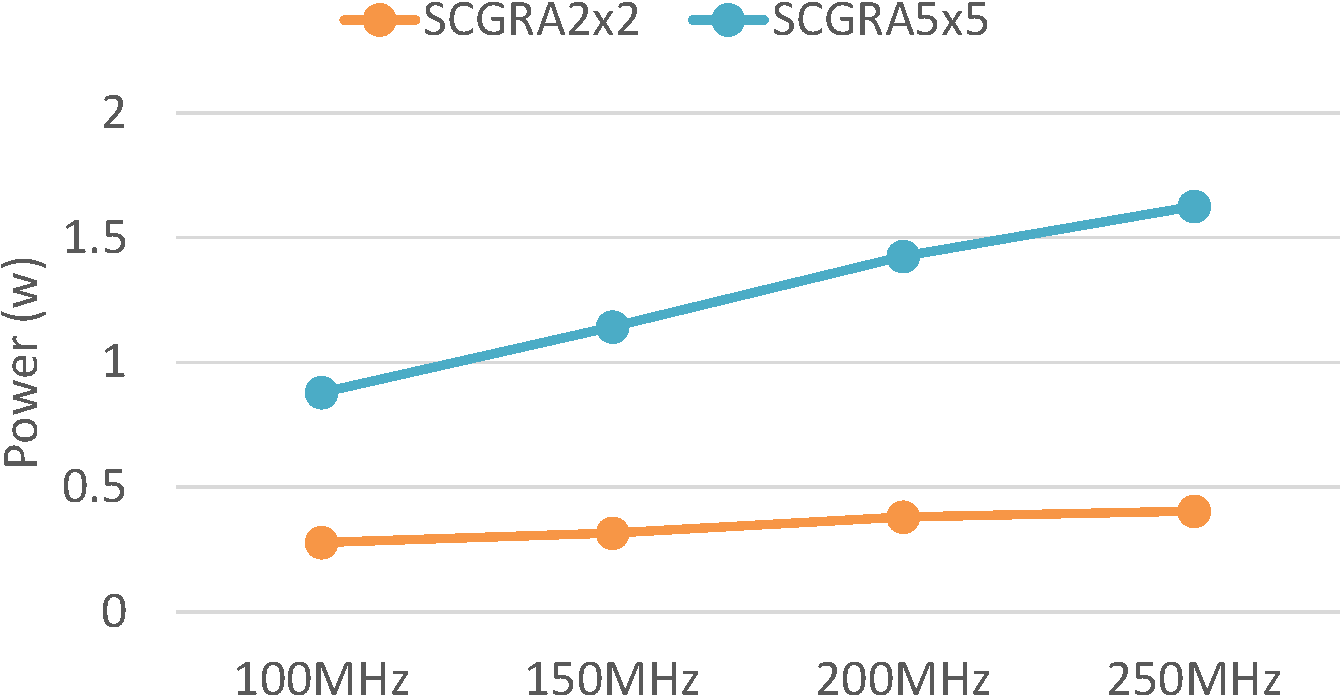
\includegraphics[width=0.5\linewidth]{pipeline-power}}
\caption{Power Consumption of SCGRA Overlays with Different Pipelining}
\label{fig:pipeline-power}
\end{figure} 

\begin{figure}[htb]
\centering
\subfigure[SCGRA$2 \times 2$]{
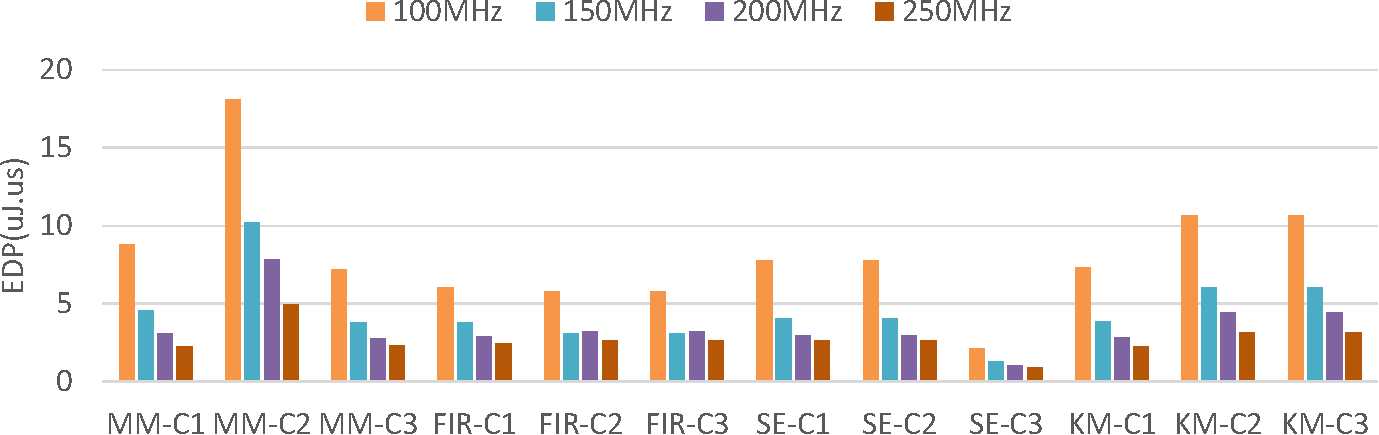
\includegraphics[width=0.8\linewidth]{pipeline-scgra2x2-edp}
\label{fig:pipeline-scgra2x2-edp}
}
\hfill
\subfigure[SCGRA $5 \times 5$]{
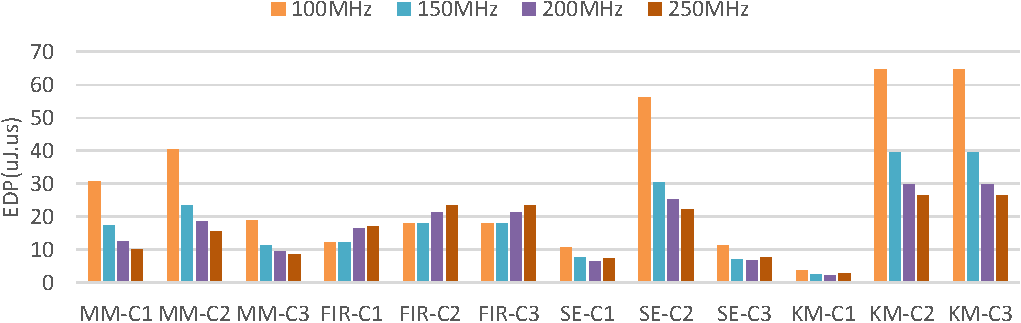
\includegraphics[width=0.8\linewidth]{pipeline-scgra5x5-edp}
\label{fig:pipeline-scgra5x5-edp}
}
\caption{Energy Delay Product of SCGRA Overlays with Different Pipelining}
\label{fig:pipeline-edp}
\end{figure}

According to the experiments in this section, highly pipelined SCGRA overlays with high implementation frequency exhibit competitive performance and energy efficiency consuming slightly more FPGA resources. Consequently, highly pipelined SCGRA overlays are used in the rest of this work.
 
\subsection{Scalability}
In this subsection, we studied the scalability of the proposed overlay architecture in terms of problem size as well as processing array size in anticipation for future FPGA devices.

To study the effect of problem size on the overlay performance, MM with matrix sizes ranging from $4\times 4$ to $20 \times 20$ were used. In the case of SCGRA overlay, \num{3} different SCGRA sizes were studied: $2\times 2$, $5\times 5$, $10\times 10$. They were targeted at the larger \texttt{zc706} FPGA with abundant hardware resource. In the case of direct HLS synthesis, Vivado HLS 2014.3 was used. \num{2} scenarios were considered. In the first scenario, the matrix multiplication was fully unrolled regardless of the resource consumption, which leads to the best achievable performance using HLS. The resulting design is labeled as HLS-FU. In the second scenario, a best-effort loop unrolling that results in maximum performance under hardware constraints was used. The design is labeled as HLS-BEU. In the case of the SCGRA overlay, the MM operations were fully unrolled. \figref{fig:mm-sim-perf} shows the number of cycles of MM execution on the resulting accelerators generated by both design methods. Communication cost was not taken into account as they remain comparable in both cases.

\begin{figure}
\centering
\subfigure[]{
\label{fig:mm-sim-perf1}
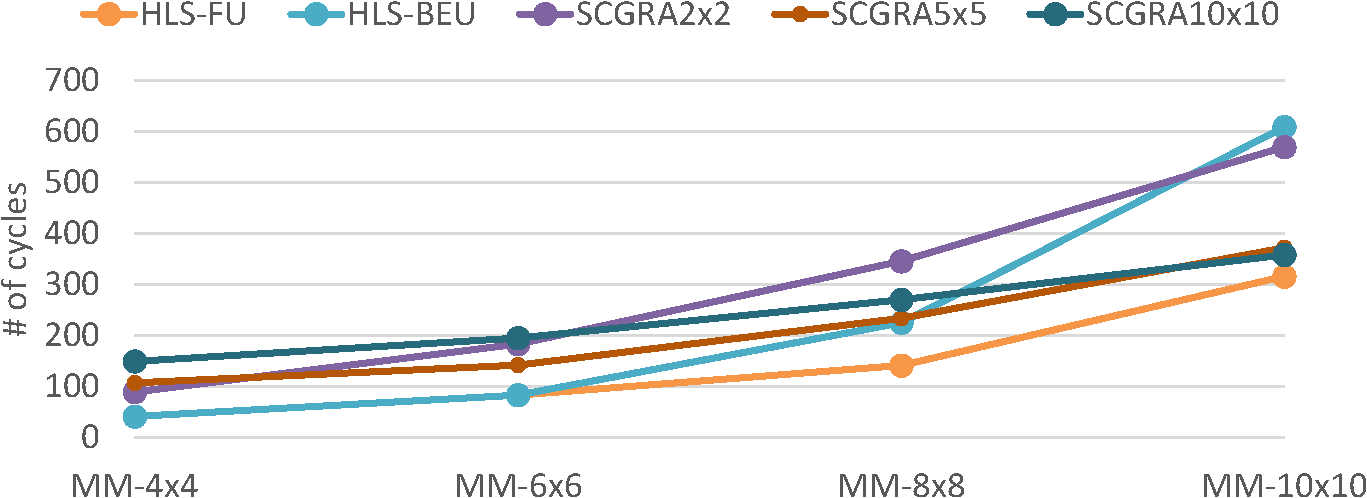
\includegraphics[width=0.7\linewidth]{mm-sim-perf1}}
\hfill
\subfigure[]{
\label{fig:mm-sim-perf2}
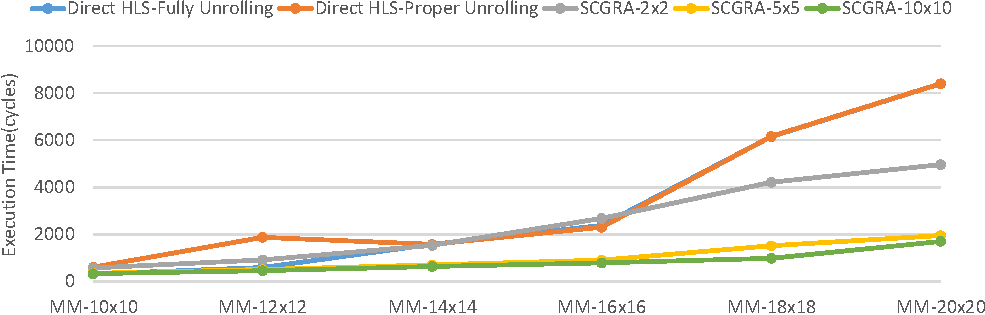
\includegraphics[width=0.7\linewidth]{mm-sim-perf2}}
\caption{\# of cycles of MM Execution on Both HLS Based Design and SCGRA Overlay}
\label{fig:mm-sim-perf}
\end{figure}

Results from the figure show that accelerators using direct HLS based design framework perform much better than the SCGRA overlay when the matrix size is small enough for the loops to be fully unrolled. However, as the matrix size grows, direct HLS can no longer afford the hardware overhead for intensive loop unrolling, limiting the performance of the resulting accelerators. As shown in \figref{fig:loop-unroll-and-pipeline}, the DSP resource consumption increases significantly with additional unrolling in return for higher performance as the matrix size increases.  While it is possible for an expert to start manually time-sharing the resources, we did not explore such sophisticated implementation technique in attempt to maintain a comparable design effort.

\begin{figure}
\center{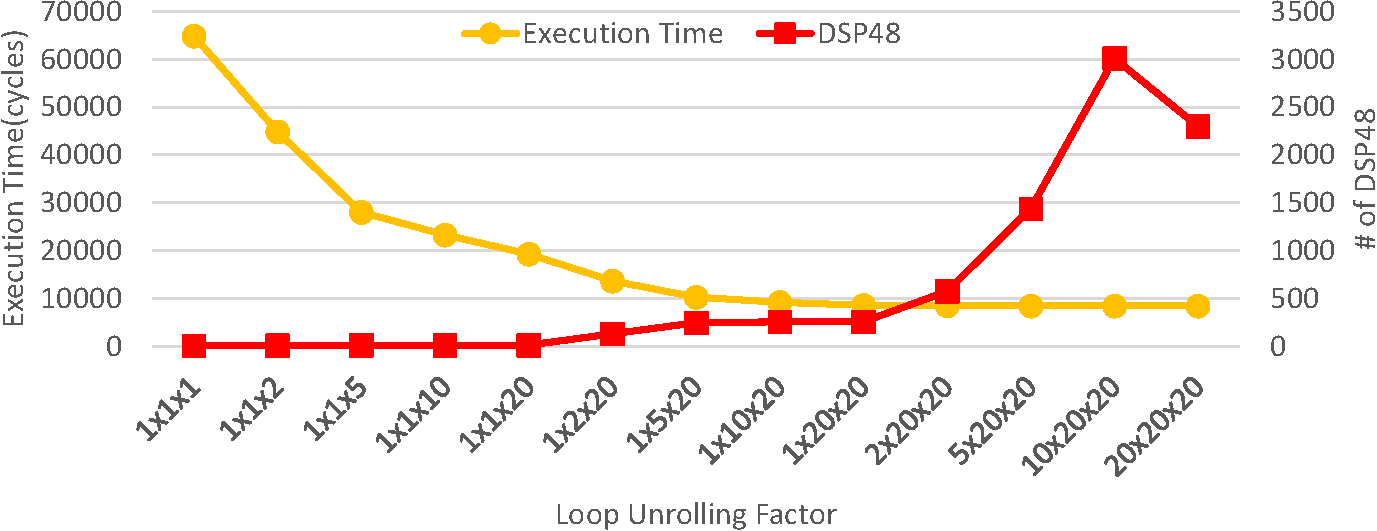
\includegraphics[width=0.7\linewidth]{hls-loop-unroll}}
\caption{MM 20x20 Implemented Using Direct HLS with Various Loop Unrolling}
\label{fig:loop-unroll-and-pipeline}
\end{figure}

On the other hand, the SCGRA overlay can naturally accommodate intensive loop unrolling through time-sharing of hardware resources. It is therefore capable of accelerating much larger portion of computation with relative ease. Its performance is mainly limited by the on-chip memory serving as instruction ROMs. In our experiments with MM that target the larger \texttt{zc706} device, MM-8x8 is the crossover point that SCGRA overlay begins to outperform.  As a comparison, the crossover point on the originally targeted Zedboard was much smaller because of the limited hardware resource.

To further study the scalability of the proposed SCGRA overlay, the performance of processing array with increasing size was experimented using MM-20x20 as an example. \figref{fig:performance-scalability} shows that in general, the additional processing power provided by the larger arrays results in better performance as expected. The performance gain reduces as the array size increases to a point when there simply is not enough available compute operations to be scheduled. This point of reflection depends on the nature of the user application. In the case of MM, the $5 \times 5$ array provided the near-optimal performance with reasonable amount of PEs.

\begin{figure}
\centering
\subfigure[Performance]{\label{fig:performance-scalability}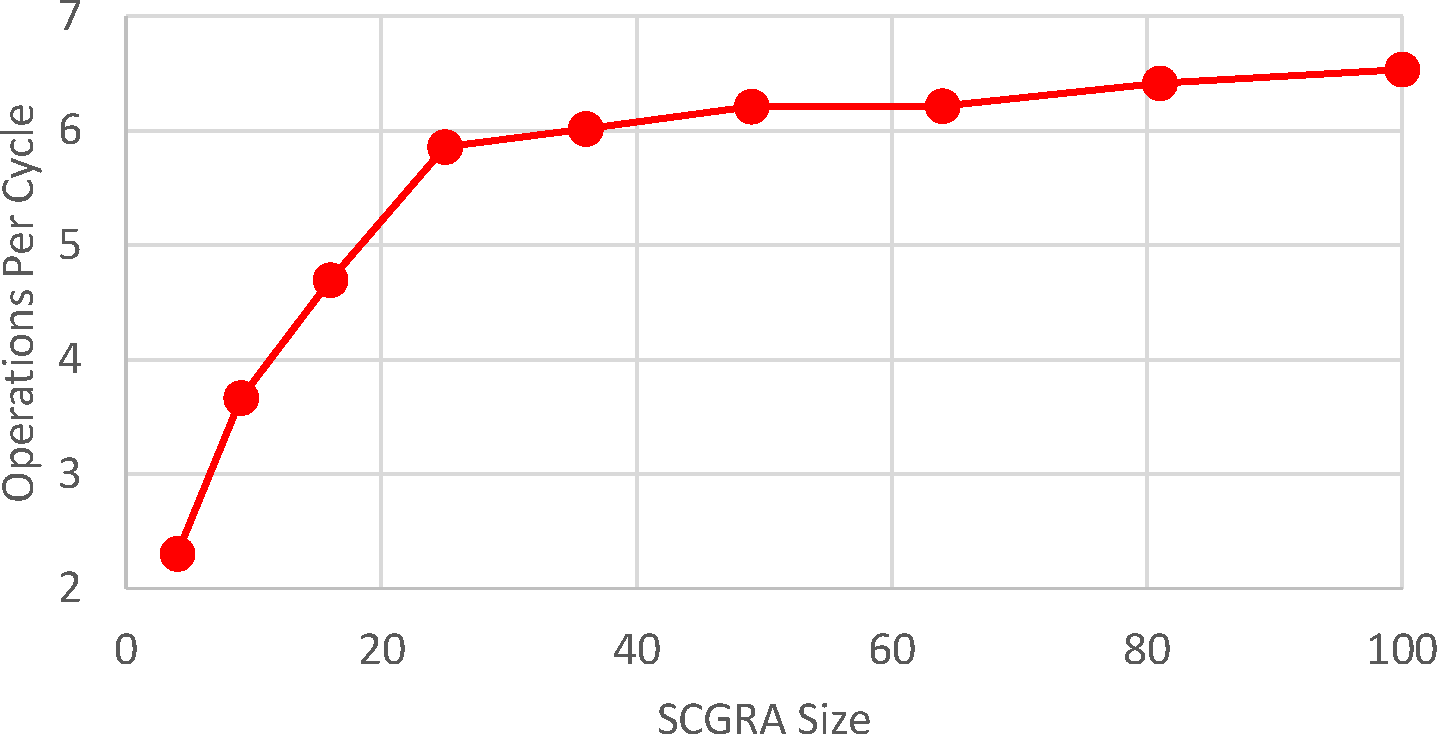
\includegraphics[width=0.45\linewidth]{perf-scale}}
\hfill
\subfigure[Resource Consumption]{\label{fig:resource-scalability}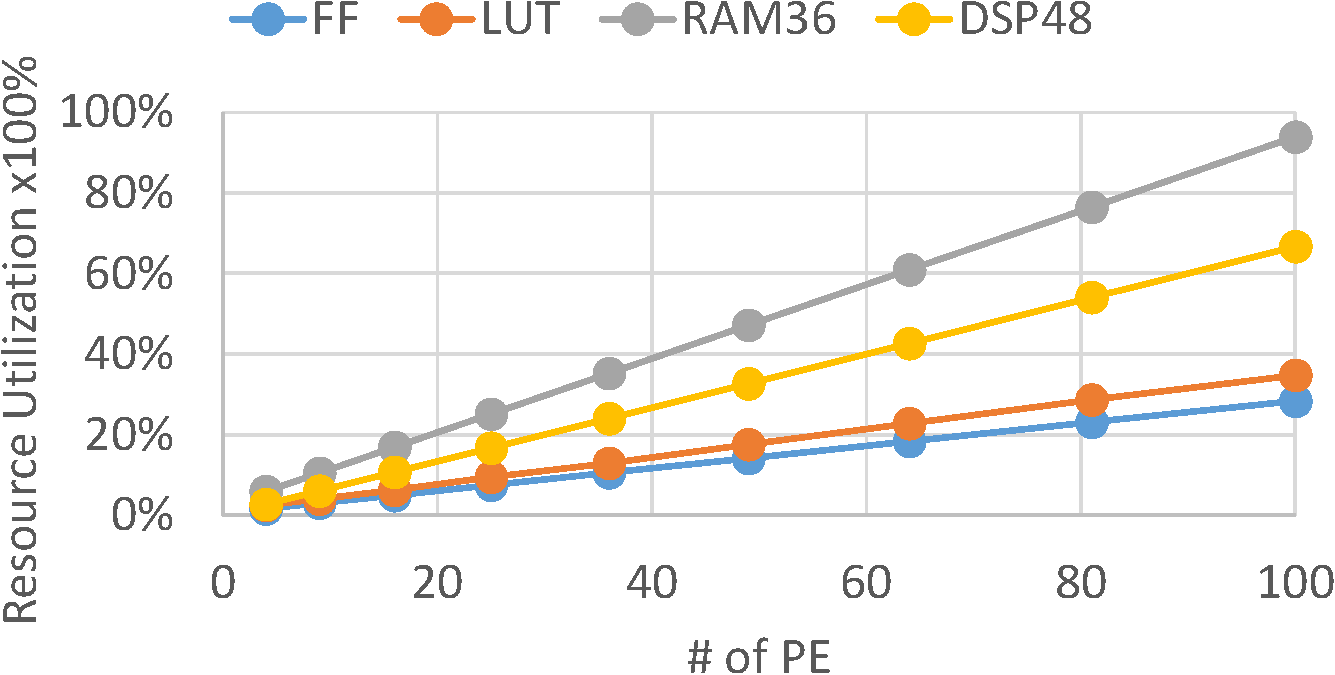
\includegraphics[width=0.45\linewidth]{resource-scalability}}
\caption{Performance, and Resource Consumption of MM-20 implemented with increasing SCGRA overlay size.}

\end{figure}

As an overlay design, it is important that its design should allow flexible scaling of its hardware resource consumption to satisfy the various resource constraints from the users. As a simple, fully synchronous and highly regular reconfigurable array, the SCGRA overlay is very much scalable in that dimension as shown in \figref{fig:resource-scalability}. From the figure, it can be seen that the hardware resource consumption associated with the SCGRA overlay increases linearly with the number of processing elements in the array.

\begin{table}[tb]
    \footnotesize
    \centering
    \caption{SCGRA Based FPGA Accelerator Configuration \label{tab:many-config}}{
        \begin{tabular}{c|c|c|c|c}
            \hline
            SCGRA Size & \tabincell{c}{Inst. Rom} & 
            \tabincell{c}{Data Mem} & \tabincell{c}{IBuf /OBuf} & 
            \tabincell{c}{Addr Buf} \\ \hline

            \tabincell{l}{2x2, 3x3, ..., 10x10} & \tabincell{l}{1k, 4k, ..., 8k}
            & 256x32 & 2kx32, 4kx32, ..., 8kx32 & 4kx16, 8kx16, ..., 16kx16 \\ \hline
        \end{tabular}
    }
\end{table}

\begin{figure}[tb]
\center{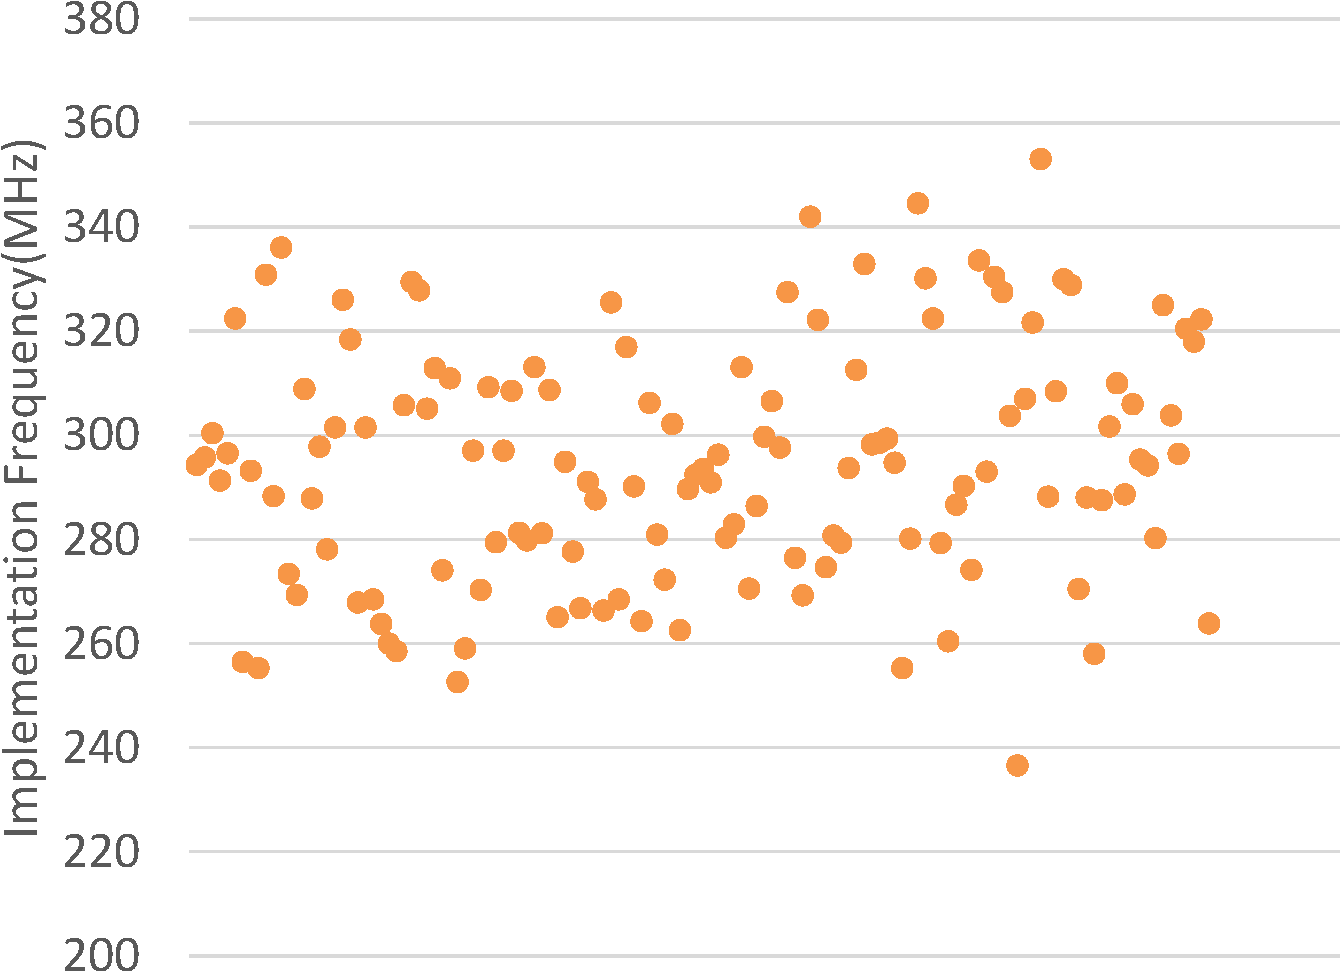
\includegraphics[width=0.6\linewidth]{impl-scale}}
\caption{fmax of SCGRA Overlay with Various Configurations}
\label{fig:impl-scale}
\end{figure}

Finally, as discussed in previous section, implementation frequency has significant influence on the performance, power consumption and energy efficiency of the resulting accelerators. Therefore, it is important to maintain high implementation frequency when the configurations of the overlay changes. To explore the scalability of the SCGRA overlay, a group of SCGRA overlays with various configurations as shown in \tabref{tab:many-config} were implemented on Zedboard. \figref{fig:impl-scale} shows the fmax of these SCGRA overlays. It can be found that the implementation frequency remains around 300MHz and stays relatively stable for various configurations.    

\section{Summary}
In this work, a template of SCGRA overlay based FPGA accelerator is developed. It is highly pipelined and exhibits higher performance and energy efficiency compared to the one with less pipeline stages. Meanwhile it is simple and easy to be extended for various applications. In addition, the regular SCGRA overlay is scalable in terms of problem size, resource consumption, implementation frequency. Particularly, the implementation frequency of the SCGRA overlay is competitive and relatively stable with various configurations.

